\section{Limits}
\label{sec:signal}

In this Section, we interpret the results of this search in terms of
the T2tt and T2bw simplified models, see Figure~\ref{fig:SigDiagram}.
Note T2tt is included at the moment, T2bw is to be added.
The branching fractions for the stop decay are assumed to be $100\%$
for each model. The signal samples are normalized to cross sections
calculated at NLO in $\alpha_S$, including the resummation of soft gluon emission at 
next-to-leading-logarithmic accuracy (NLO+NLL). 

\begin{figure}[hbt]
  \begin{center}
        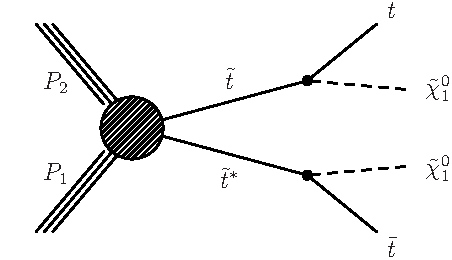
\includegraphics[width=0.5\linewidth]{plots/stopPlot/T2tt.pdf}%
        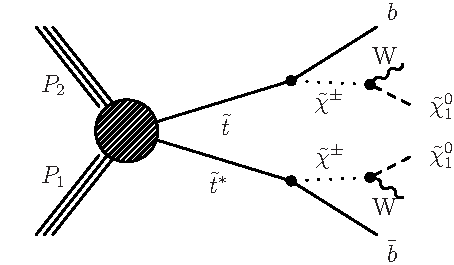
\includegraphics[width=0.5\linewidth]{plots/stopPlot/T2bw.pdf}%
	\caption{Diagram for the T2tt (left) and T2bw (right)
          simplified models.}
	\label{fig:SigDiagram}
      \end{center}
\end{figure}

The exclusion is performed using the results from the counting experiments in the signal regions
defined by \met\ and \mt\ and listed in Table~\ref{tab:srdef}. 
The cross section upper limit calculation is performed with the LandS software using the LHC-type CLs criterion. 

The signal efficiency uncertainties include the luminosity (4.4\%), lepton ID and isolation
efficiency (2\%), and trigger efficiency (3\%). The uncertainty from JES
is assessed for each scan point following the POG-recommended
procedure, by varying the jet energies by the \pt- and $\eta$-
dependent uncertainties, and propagating this to the jet multiplicity,
\met\ and \mt. The official b-tagging scale-factors for CSVM are used to compute scale
factors for the signal. The results are nearly constant across the
model parameter space, and an overall scale factor of $(98 \pm 2)\%$
is used. 

%However, it is instructive to get a first feeling for where the sensitivity of this search is.
%We do this in terms of ``expected limits'', assuming a null result.
%The case of an excess is quite different and more complicated.

The signal efficiency in the stop vs LSP mass plane for T2tt is shown 
for each signal region in Figures~\ref{fig:allsrlimits},
~\ref{fig:allsrlimits2} and~\ref{fig:allsrlimits3} (left). These distributions show how
challenging it is to have sensitivity near the kinematical boundaries.
The cross section upper limits, along with the
observed and expected exclusion contours, are also shown in
Figures~\ref{fig:allsrlimits},~\ref{fig:allsrlimits2} and~\ref{fig:allsrlimits3} (right).
The complementarity of the different signal regions is readily apparent.  
The sensitivity to low (high) stop masses comes from the 
low (high) \met\ signal regions.

\begin{figure}[hbt]
  \begin{center}
        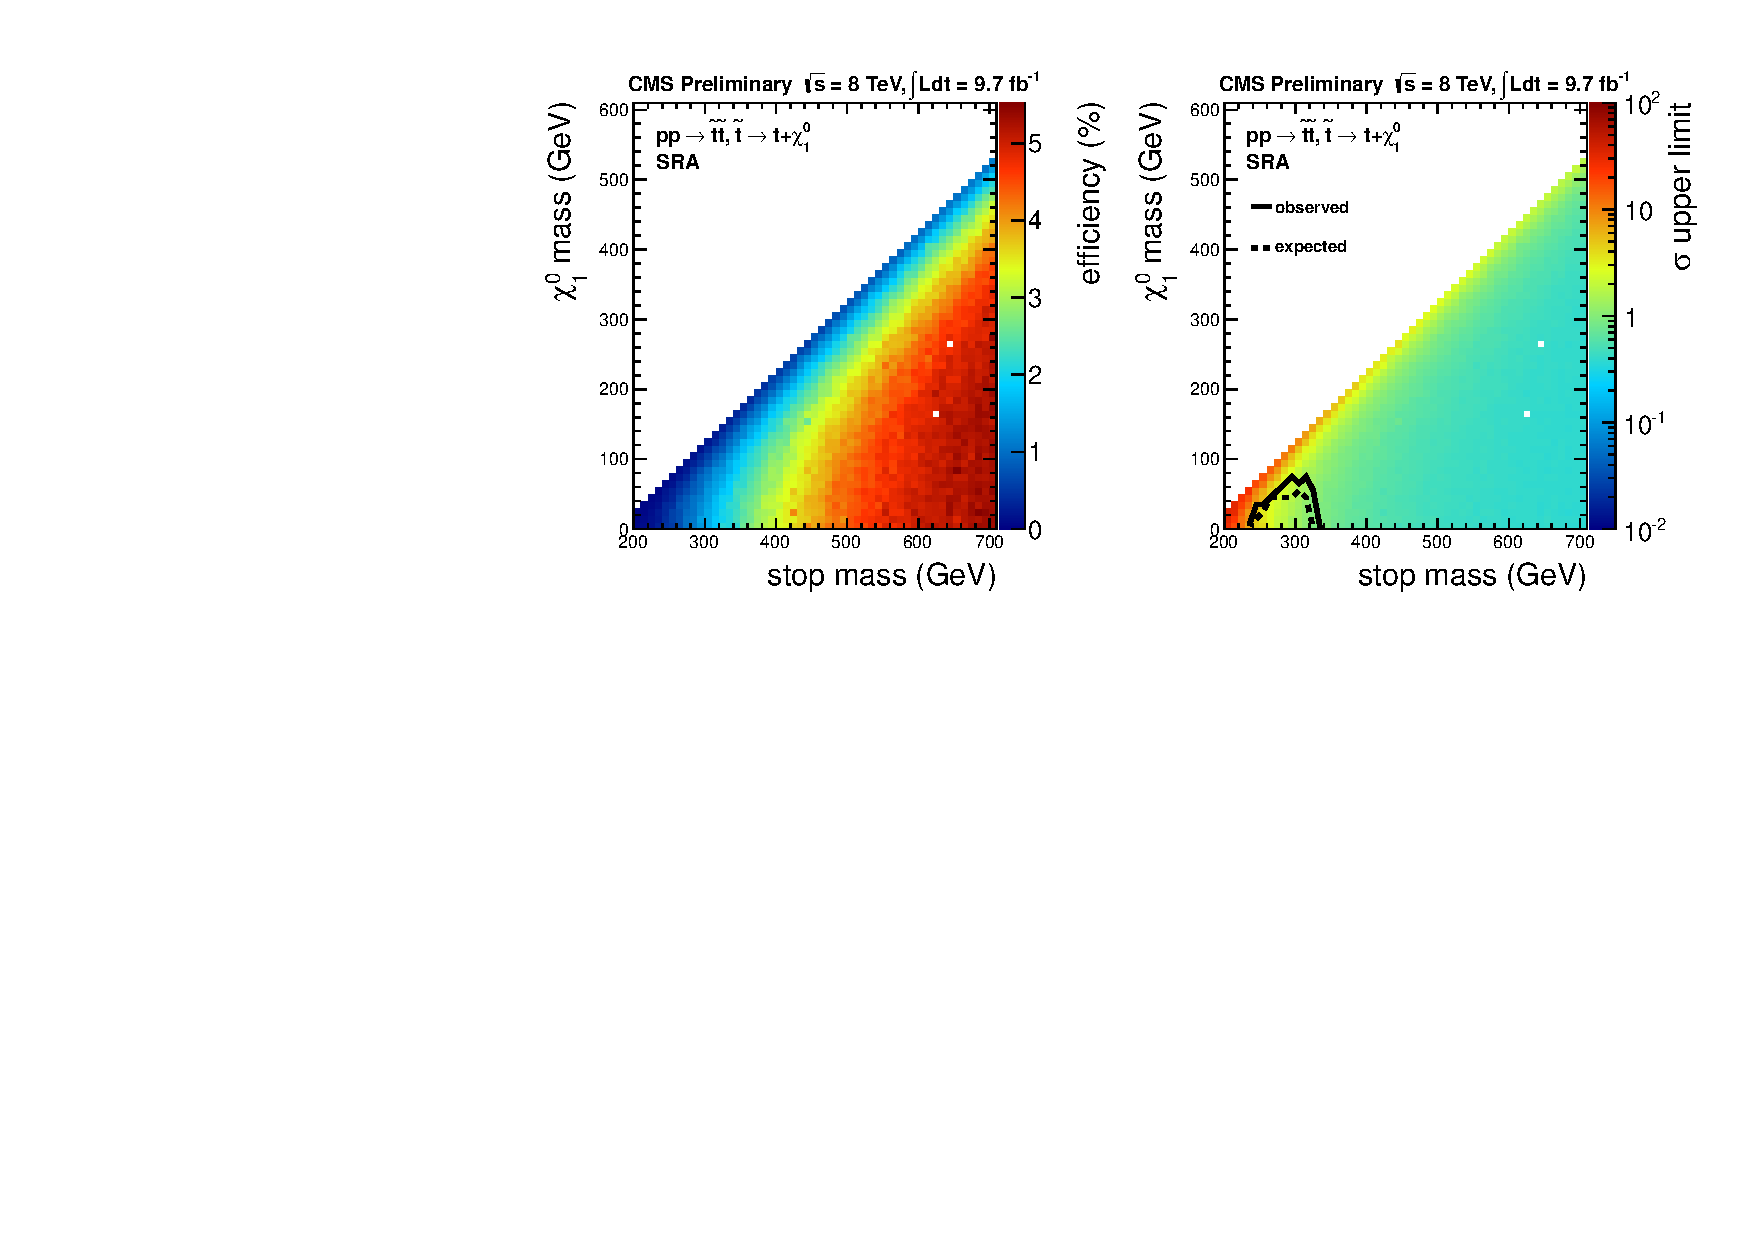
\includegraphics[width=1.\linewidth]{plots/T2tt_SRA.pdf}
        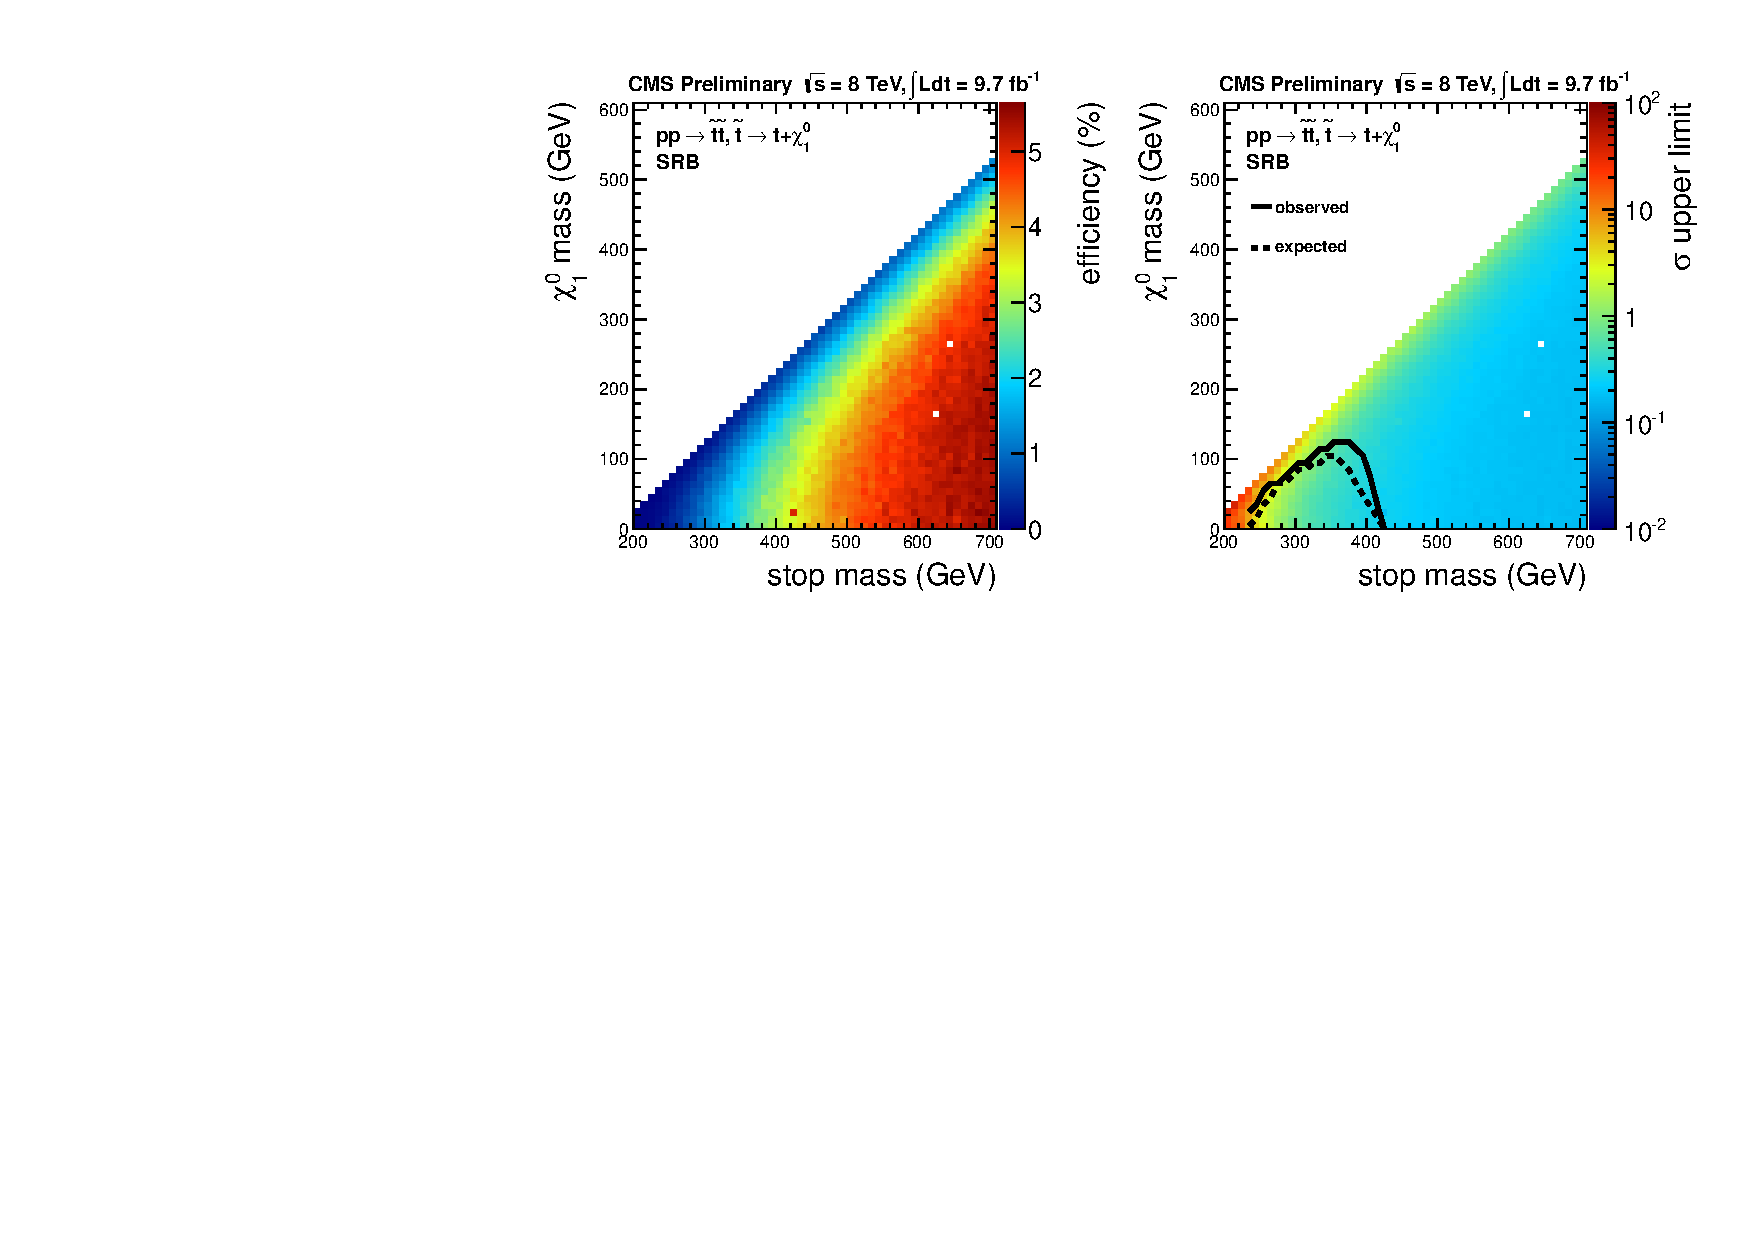
\includegraphics[width=1.\linewidth]{plots/T2tt_SRB.pdf}
        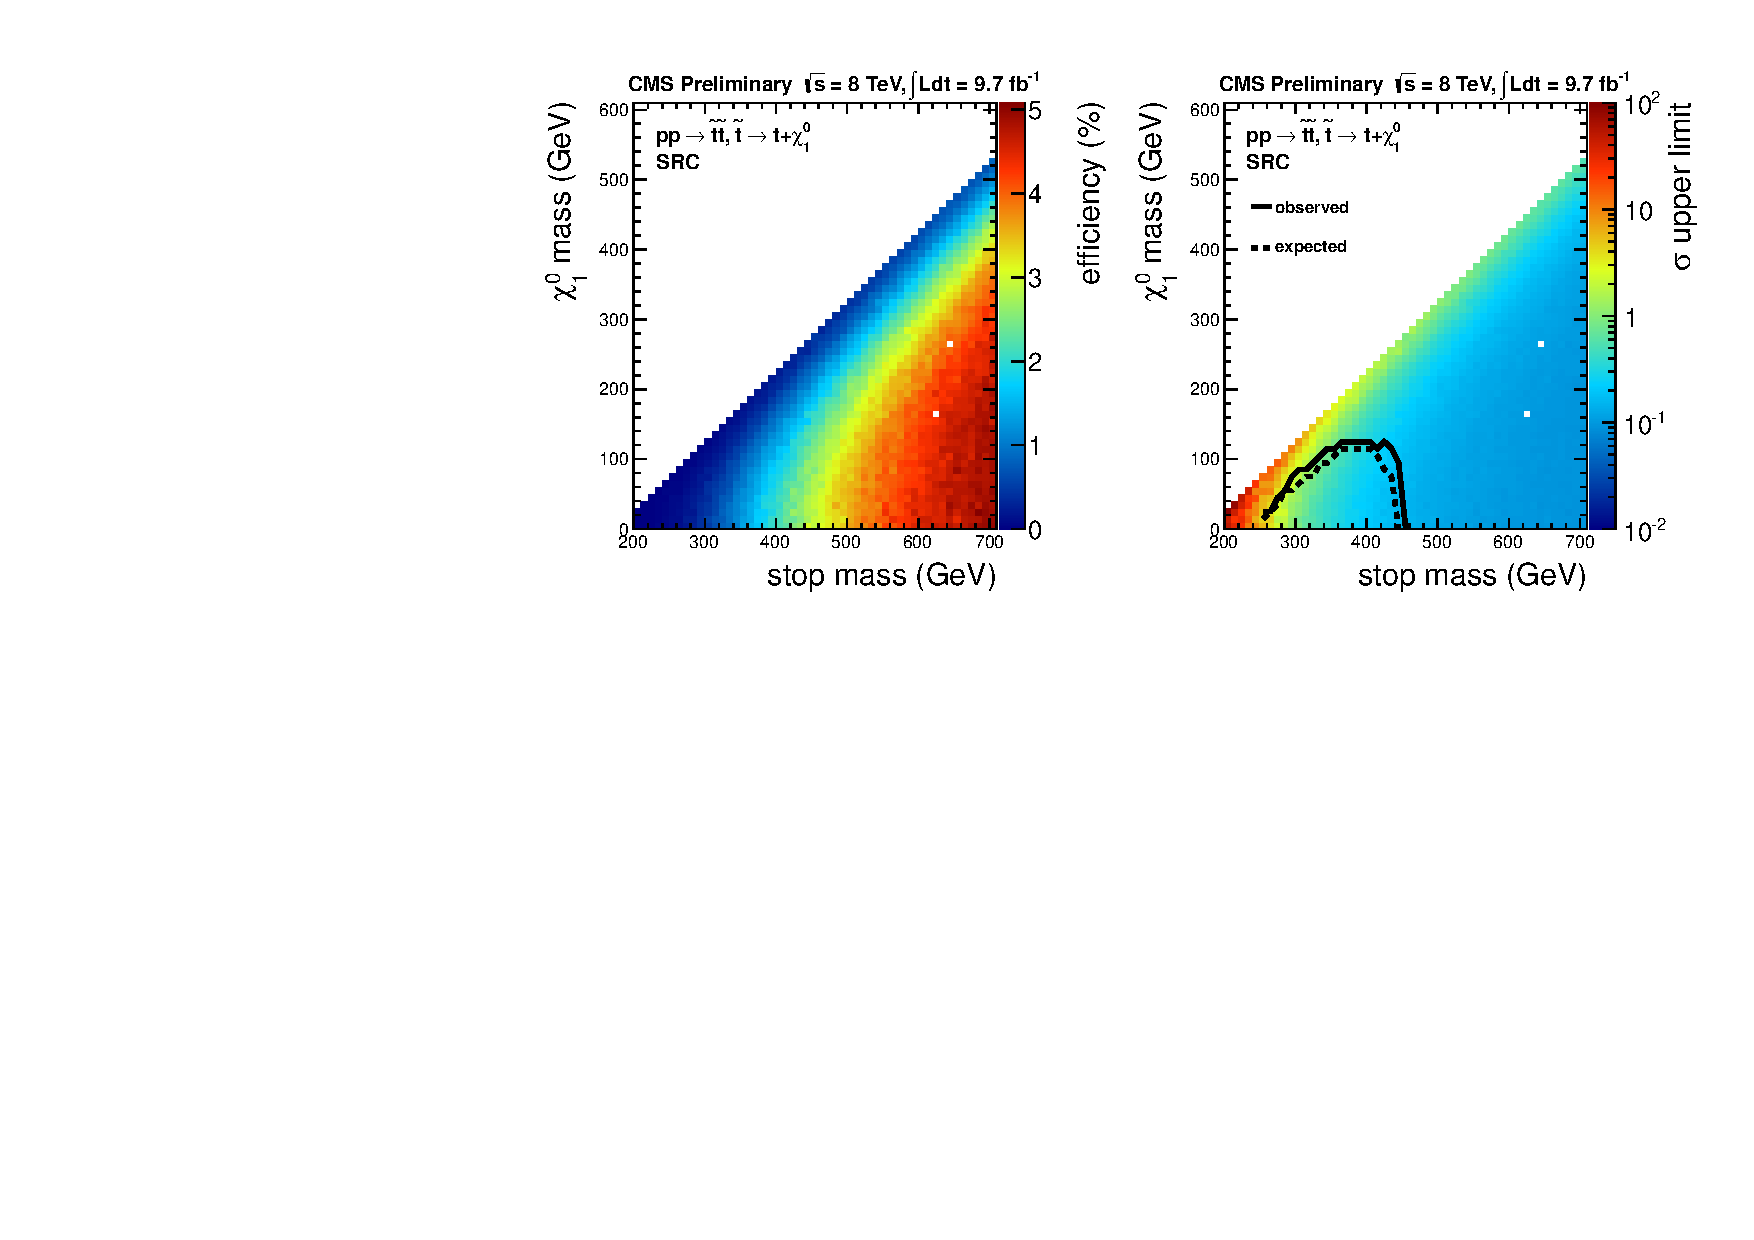
\includegraphics[width=1.\linewidth]{plots/T2tt_SRC.pdf}
    \caption{Signal efficiency (left) and cross section upper limit
      (right) for the T2tt model, showing both the expected and
      observed exclusion contours. The results for signal regions SRA (top),
      SRB (middle) and SRC (bottom) are shown separately.}
\label{fig:allsrlimits}
      \end{center}
\end{figure}

\begin{figure}[hbt]
  \begin{center}
        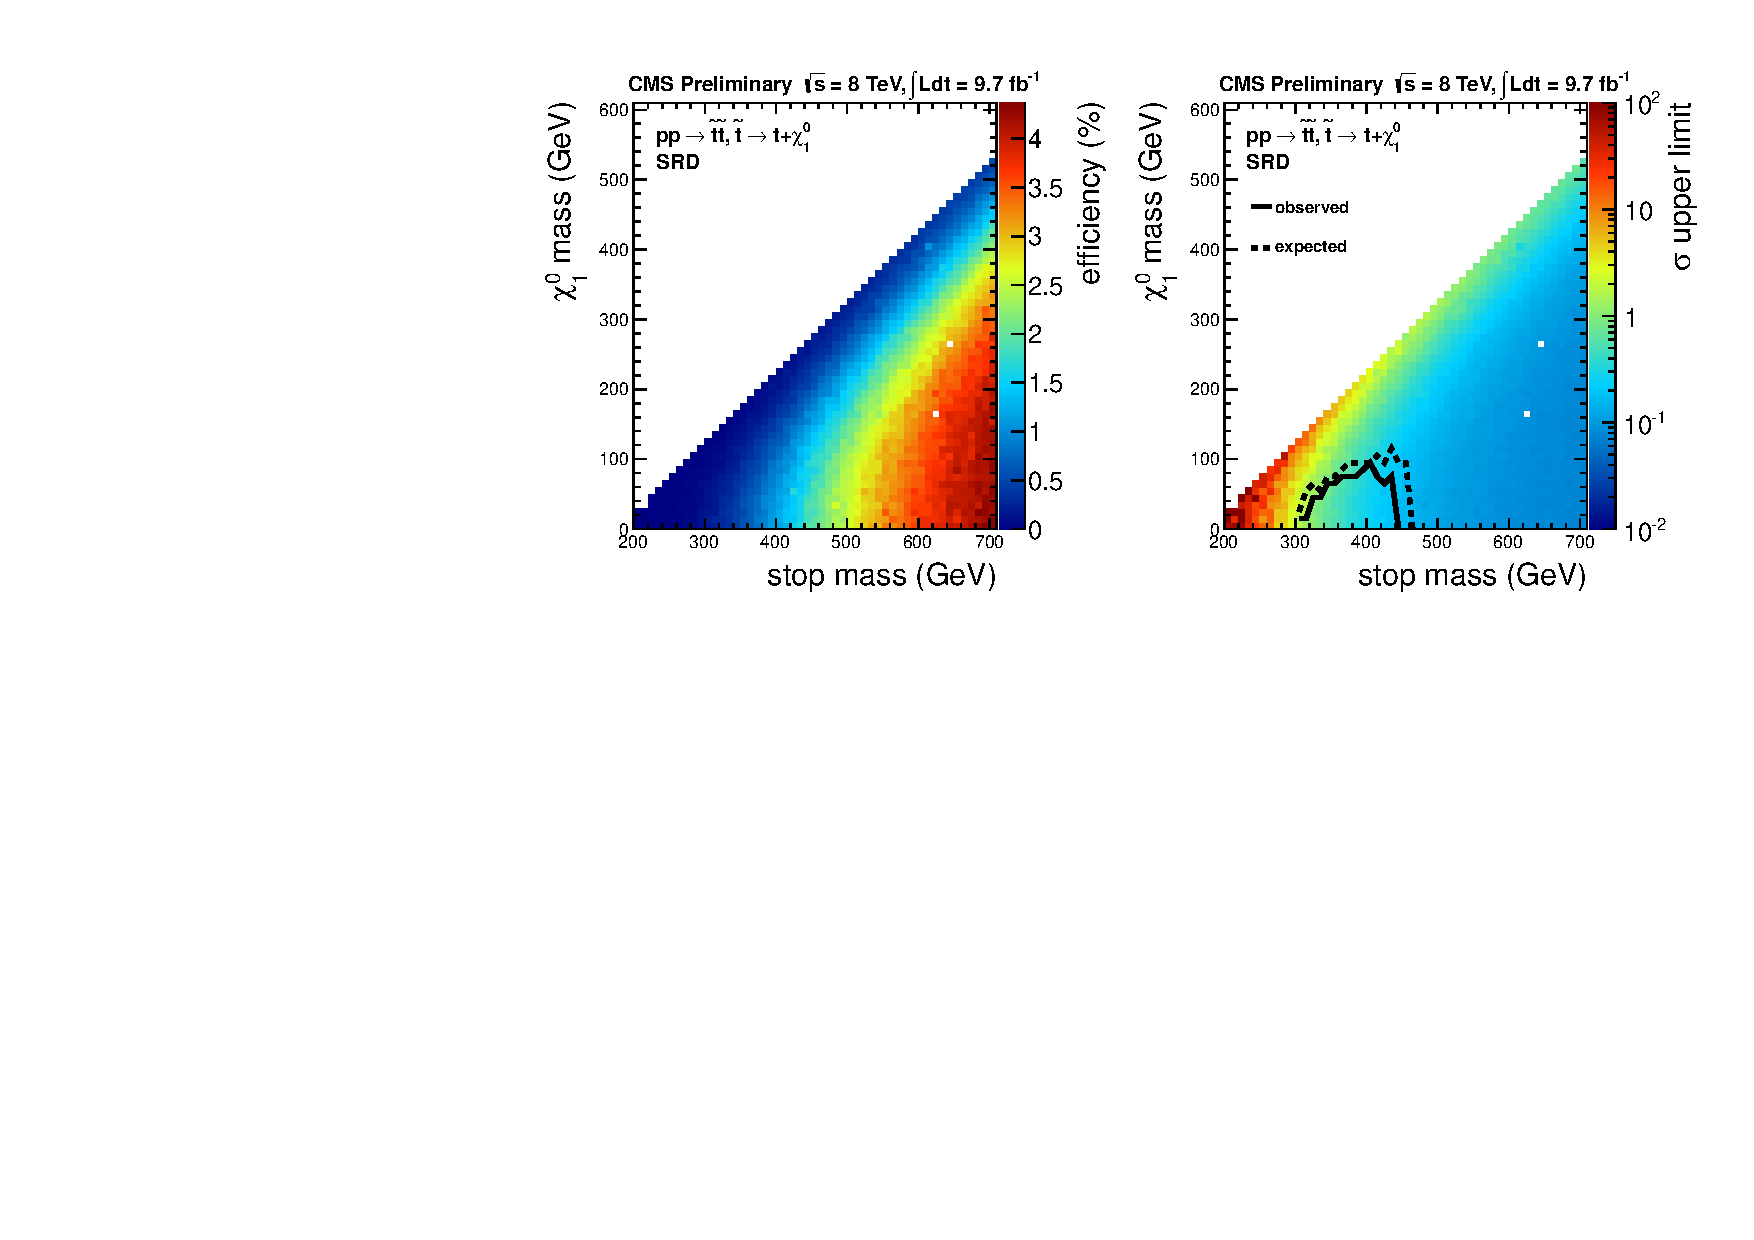
\includegraphics[width=1.\linewidth]{plots/T2tt_SRD.pdf}
        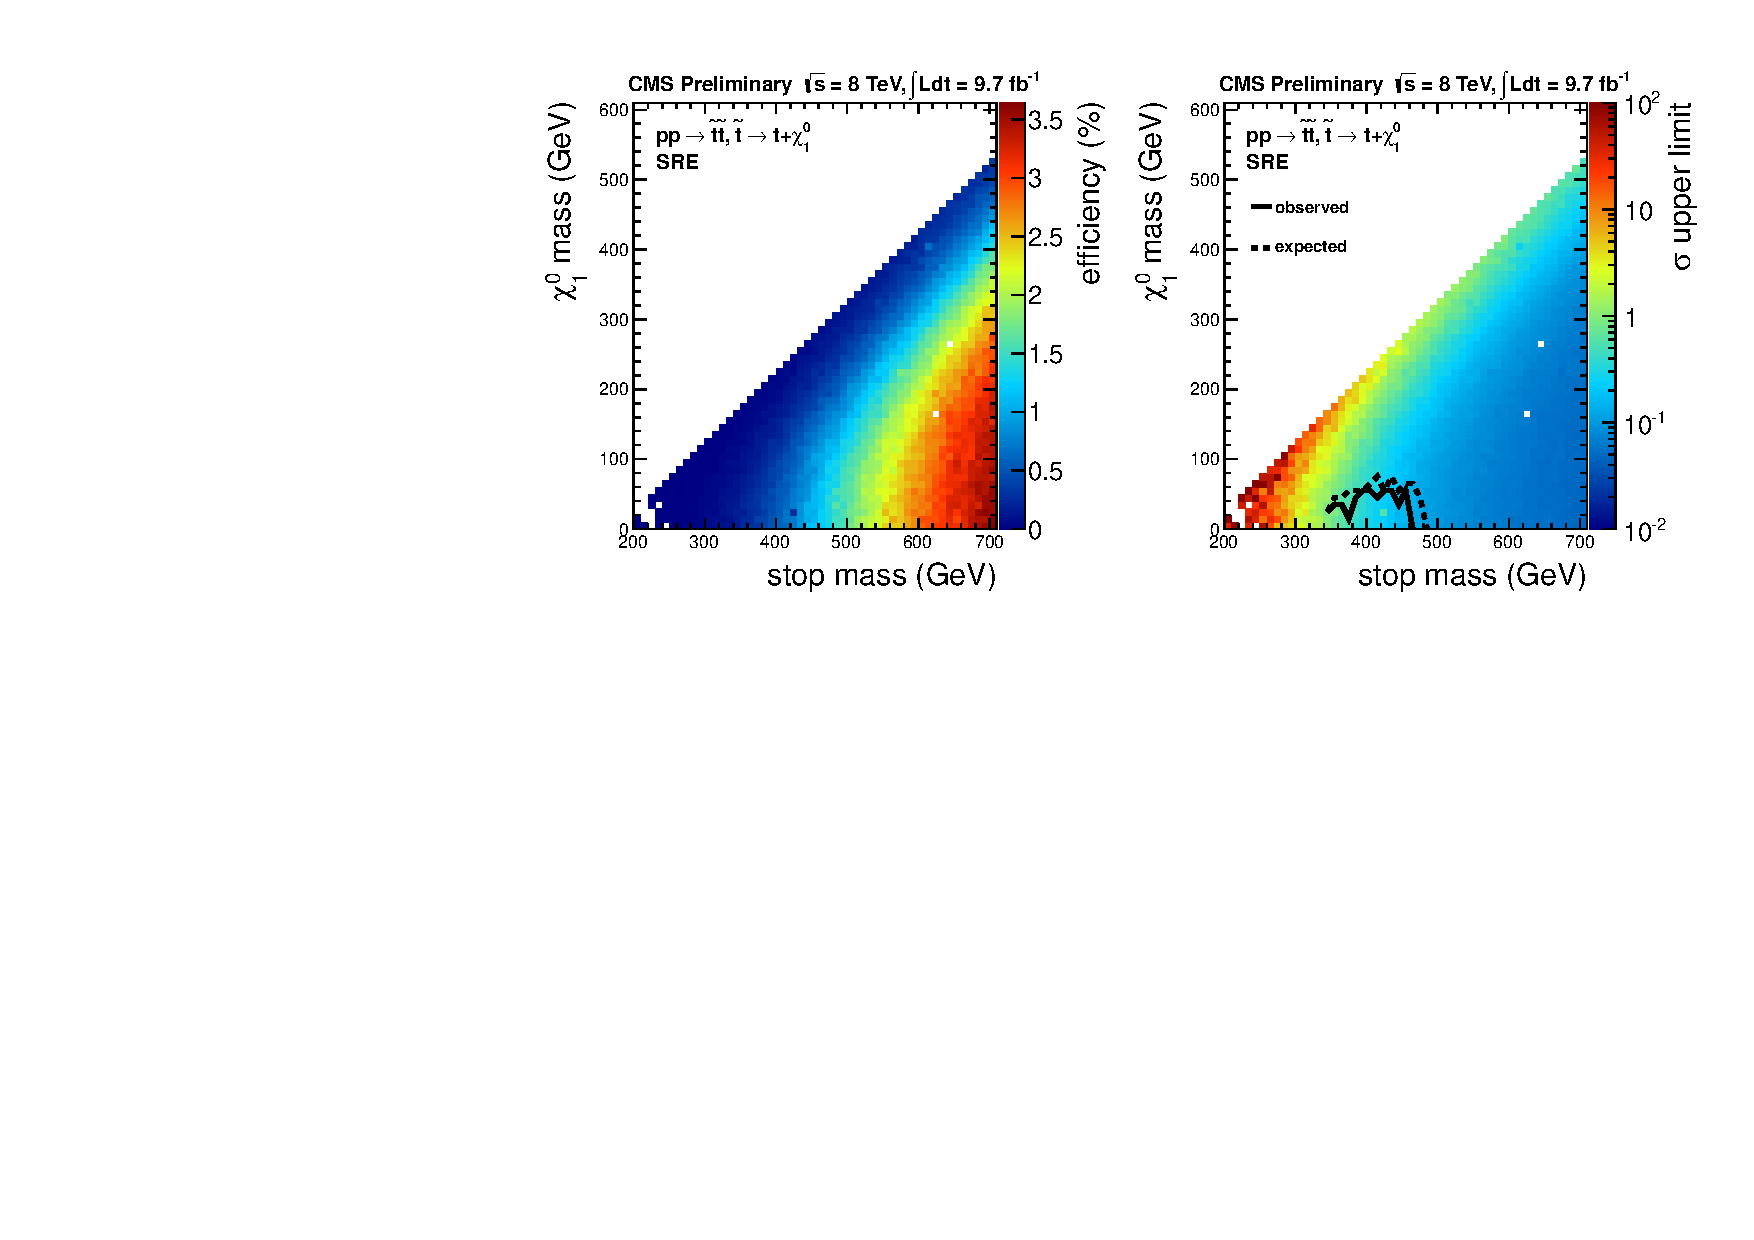
\includegraphics[width=1.\linewidth]{plots/T2tt_SRE.pdf}
    \caption{Signal efficiency (left) and cross section upper limit
      (right) for the T2tt model, showing both the expected and
      observed exclusion contours. The results for signal regions SRD (top),
      and SRE (bottom) are shown separately.}
\label{fig:allsrlimits2}
      \end{center}
\end{figure}

\begin{figure}[hbt]
  \begin{center}
        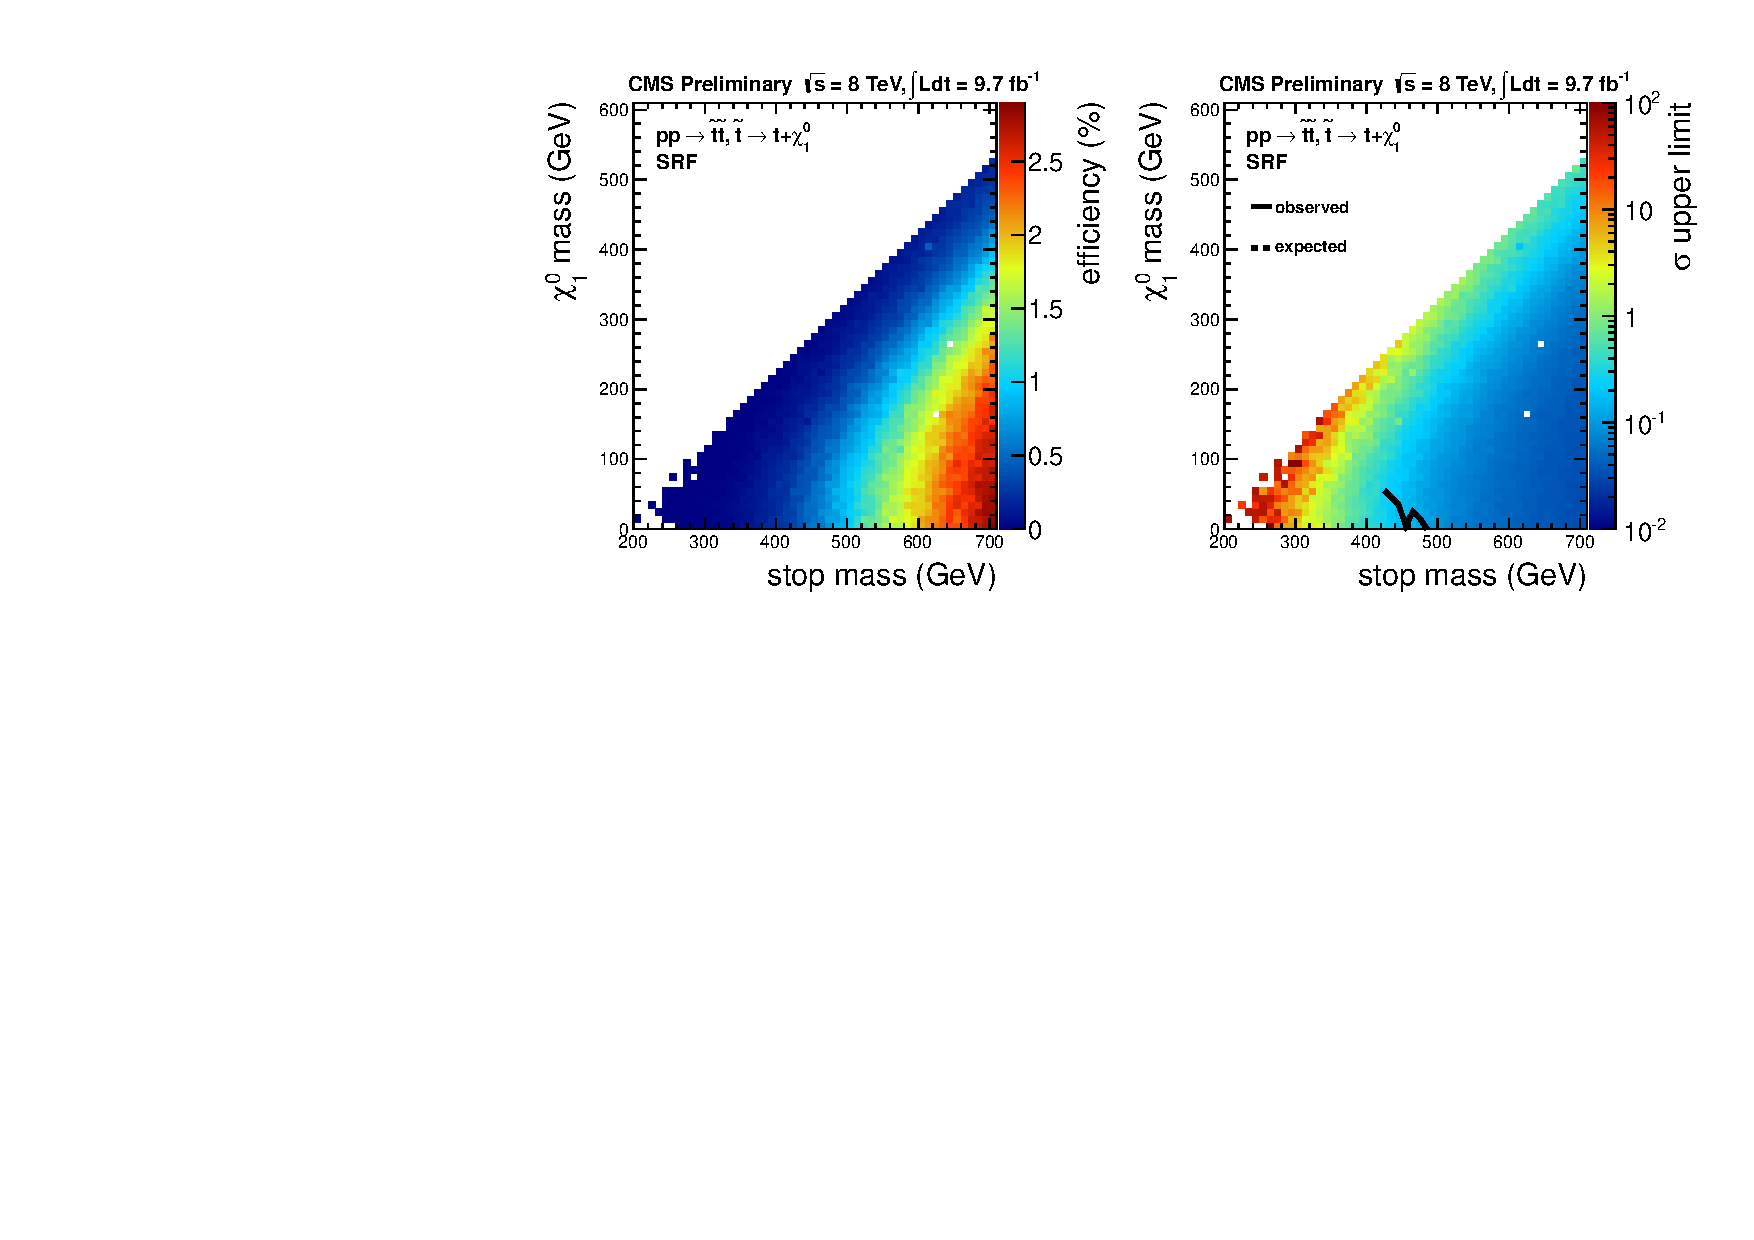
\includegraphics[width=1.\linewidth]{plots/T2tt_SRF.pdf}
        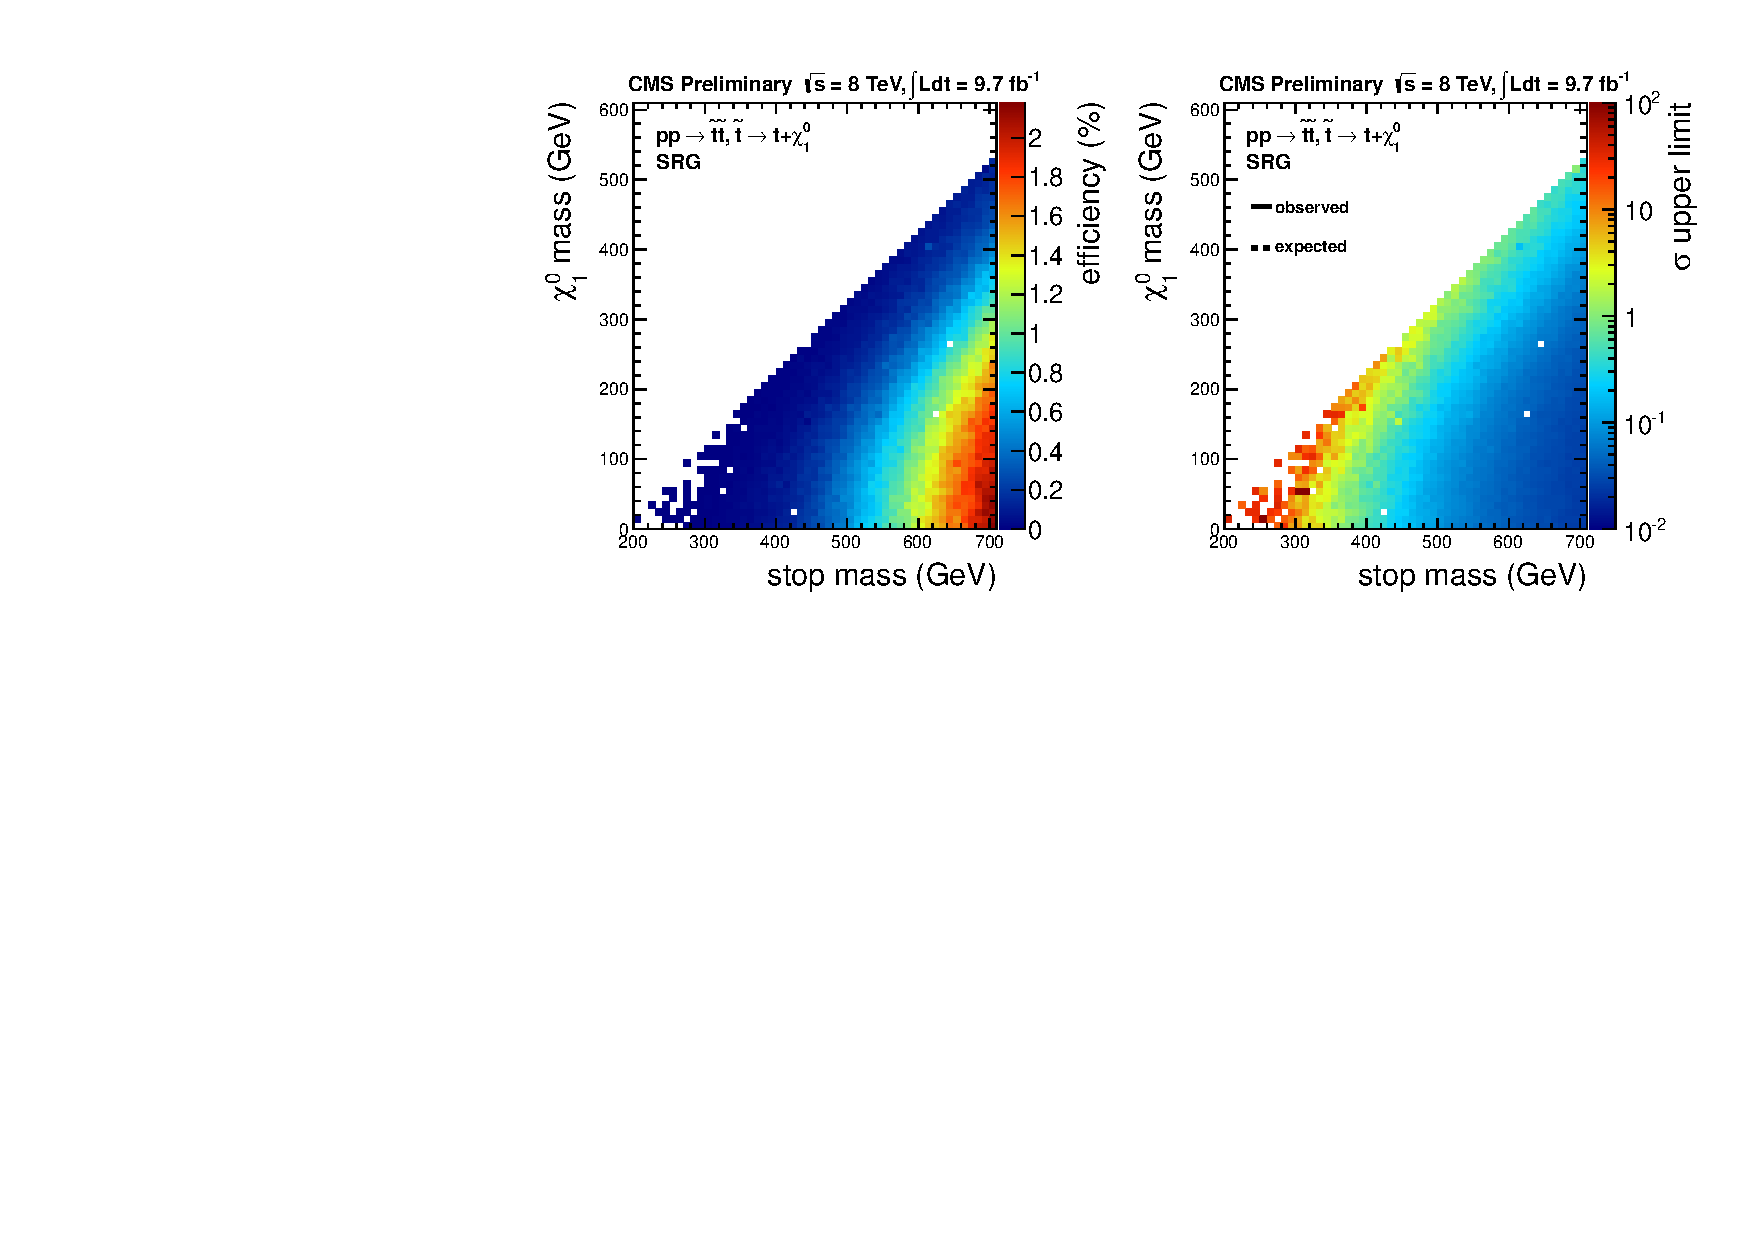
\includegraphics[width=1.\linewidth]{plots/T2tt_SRG.pdf}
    \caption{Signal efficiency (left) and cross section upper limit
      (right) for the T2tt model, showing both the expected and
      observed exclusion contours. The results for signal regions SRF (top),
      and SRG (bottom) are shown separately.}
\label{fig:allsrlimits3}
      \end{center}
\end{figure}

A combined result is obtained using the observed limit from the signal
region with the best expected limit for each scan point. The combined cross
section upper limits, with the observed and expected exclusion contours, are
shown in Figure~\ref{fig:comblimit} (left).
%The combination is performed by selecting at each scan point the
%observed limit from the signal region with the best expected limit.
The signal region with the best expected limit for each scan point is
also shown in Figure~\ref{fig:comblimit} (right). This search probes
stops in the T2tt scenario with masses in the range 250 GeV to 450 GeV for LSP masses up to
about 110 GeV.

 \begin{figure}[hbt]
  \begin{center}
       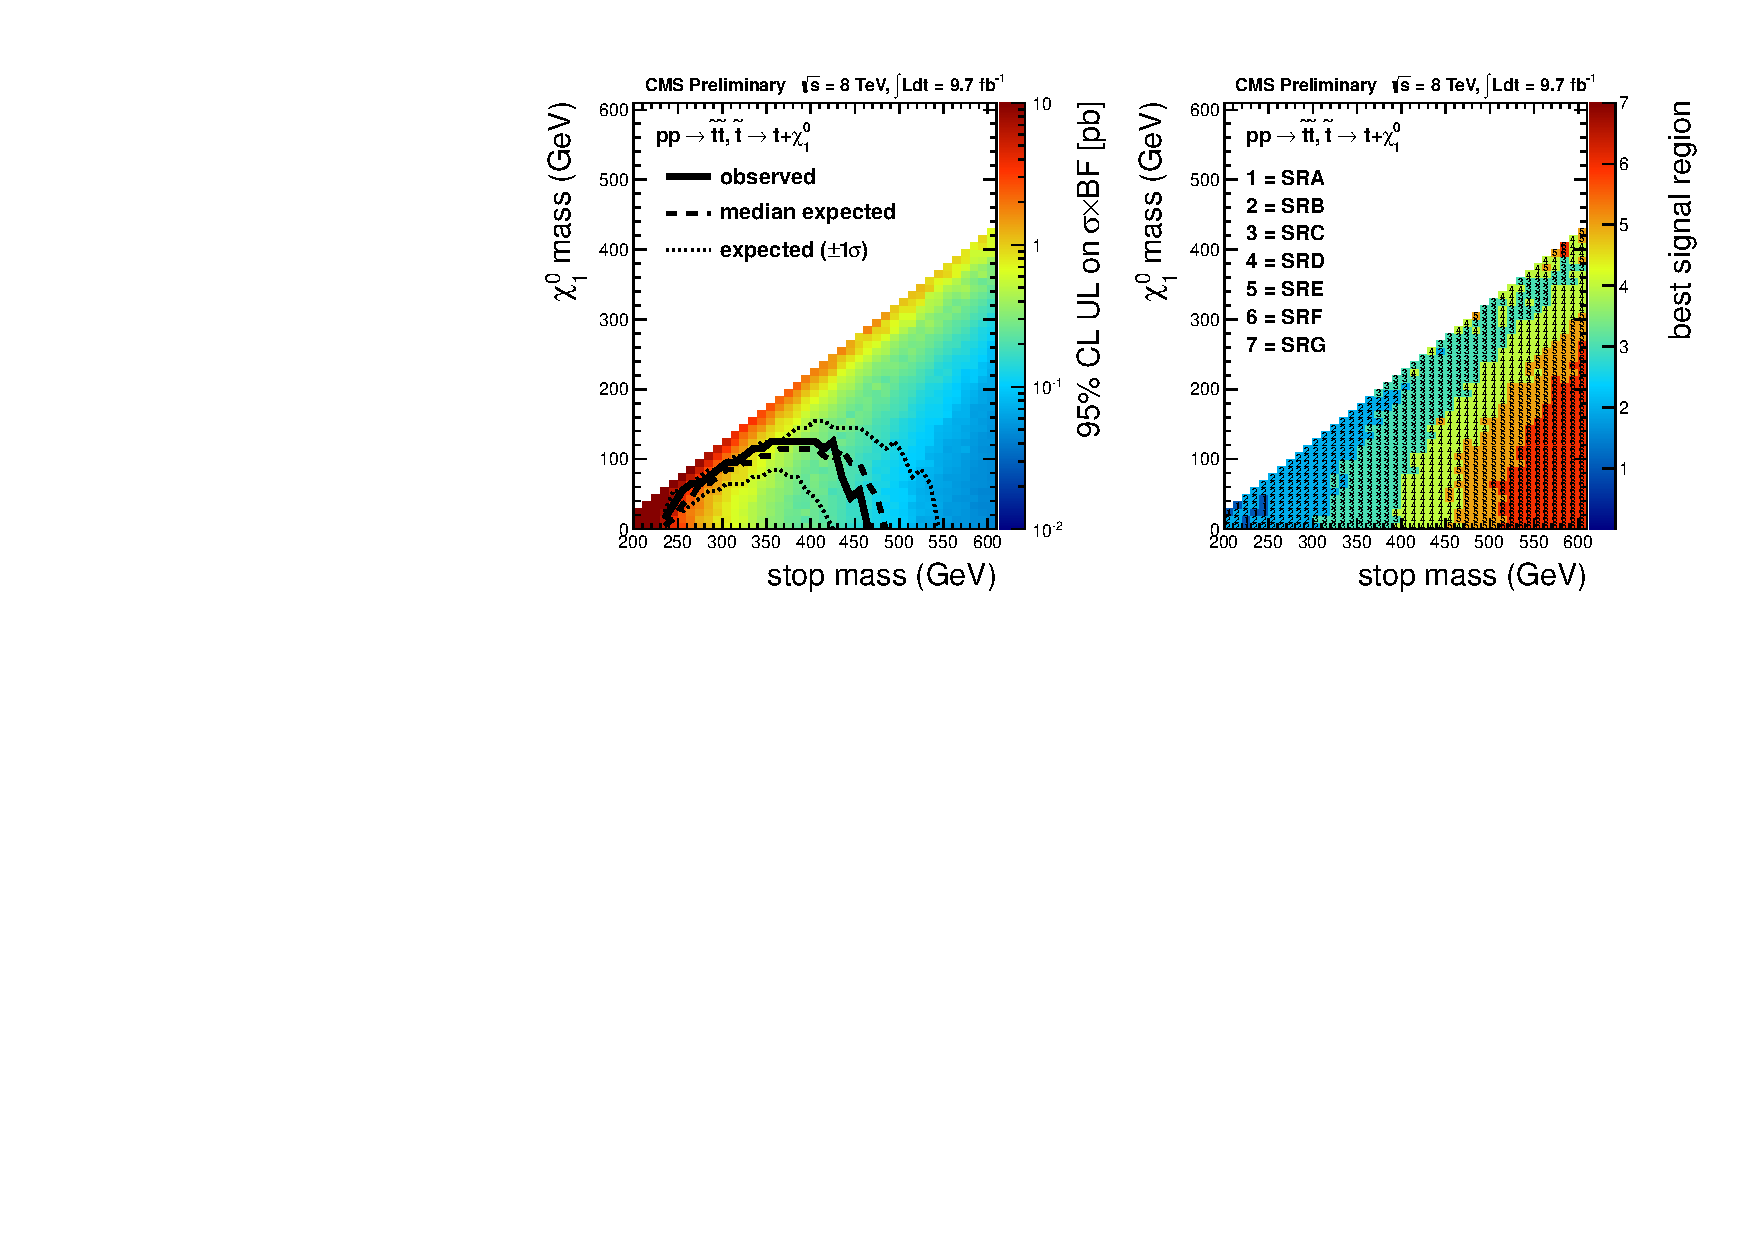
\includegraphics[width=1.\linewidth]{plots/T2tt_combined.pdf}%
    \caption{Upper limit on the cross section for the T2tt model in
      the plane of stop vs. LSP mass, showing
      both the expected (dashed) and observed (solid curve) exclusion
      contours (left). The observed
      limit is selected from the signal region with the best expected
      limit (shown on right). All uncertainties are included and the
      dotted contours around the dashed expected limit correspond to
      the $\pm 1\sigma$ result.}
\label{fig:comblimit}
      \end{center}
\end{figure}

%\begin{figure}[hbt]
%  \begin{center}
%        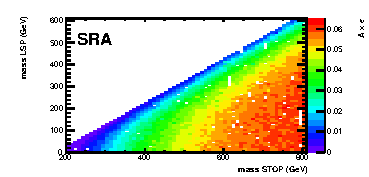
\includegraphics[width=0.5\linewidth]{plots/stopPlot/massesA_eff.pdf}%
%        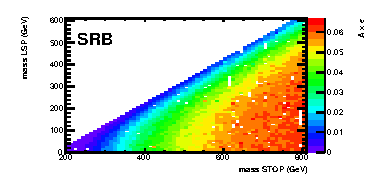
\includegraphics[width=0.5\linewidth]{plots/stopPlot/massesB_eff.pdf}
%        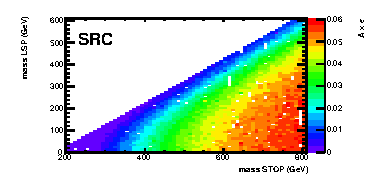
\includegraphics[width=0.5\linewidth]{plots/stopPlot/massesC_eff.pdf}%
%        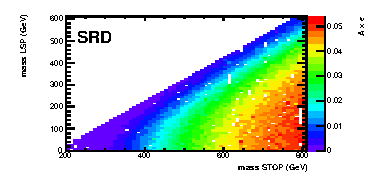
\includegraphics[width=0.5\linewidth]{plots/stopPlot/massesD_eff.pdf}
%        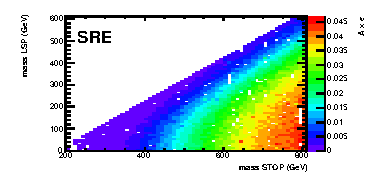
\includegraphics[width=0.5\linewidth]{plots/stopPlot/massesE_eff.pdf}%
%        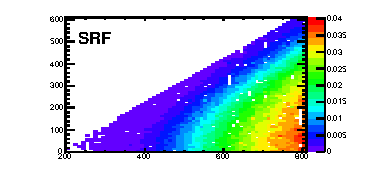
\includegraphics[width=0.5\linewidth]{plots/stopPlot/massesF_eff.pdf}
%        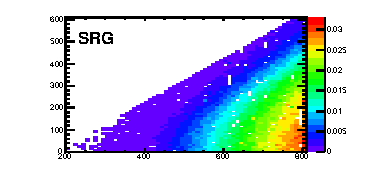
\includegraphics[width=0.5\linewidth]{plots/stopPlot/massesG_eff.pdf}%
%    \caption{Signal efficeincy in for the T2tt }
%\label{fig:SigEff}
%      \end{center}
%\end{figure}
%
%\begin{figure}[hbt]
%  \begin{center}
%        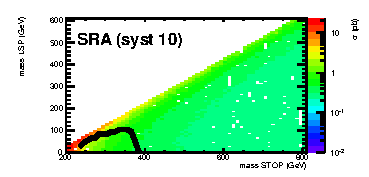
\includegraphics[width=0.5\linewidth]{plots/stopPlot/masses_SRA_xsecO.pdf}%
%        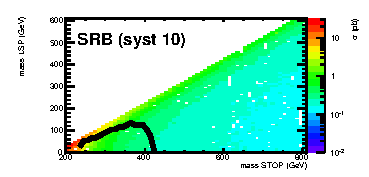
\includegraphics[width=0.5\linewidth]{plots/stopPlot/masses_SRB_xsecO.pdf}
%        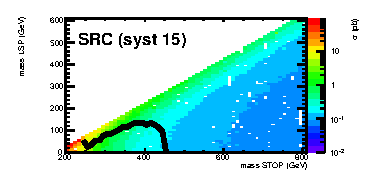
\includegraphics[width=0.5\linewidth]{plots/stopPlot/masses_SRC_xsecO.pdf}%
%        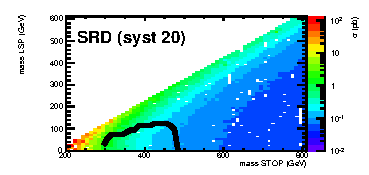
\includegraphics[width=0.5\linewidth]{plots/stopPlot/masses_SRD_xsecO.pdf}
%        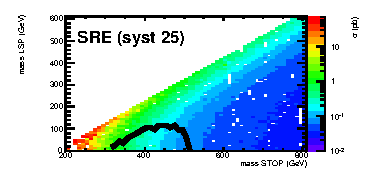
\includegraphics[width=0.5\linewidth]{plots/stopPlot/masses_SRE_xsecO.pdf}%
%        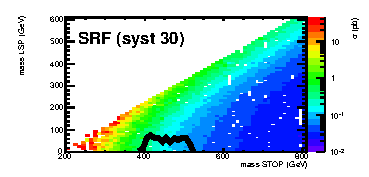
\includegraphics[width=0.5\linewidth]{plots/stopPlot/masses_SRF_xsecO.pdf}
%        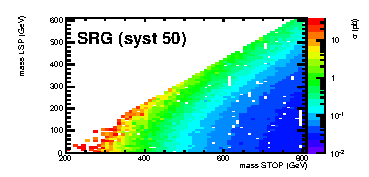
\includegraphics[width=0.5\linewidth]{plots/stopPlot/masses_SRG_xsecO.pdf}%
%    \caption{Expected upper limit on the cross section for the
%      T2tt. A somewhat optimistic scenario is considered as systematics on the
%      background. The assumed uncertainties on the background (in percent) is indicated on the plot.}
%\label{fig:limO}
%      \end{center}
%\end{figure}
%
%\begin{figure}[hbt]
%  \begin{center}
%        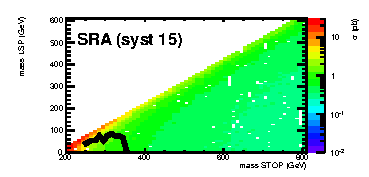
\includegraphics[width=0.5\linewidth]{plots/stopPlot/masses_SRA_xsecP.pdf}%
%        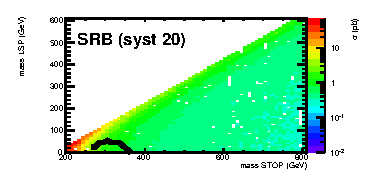
\includegraphics[width=0.5\linewidth]{plots/stopPlot/masses_SRB_xsecP.pdf}
%        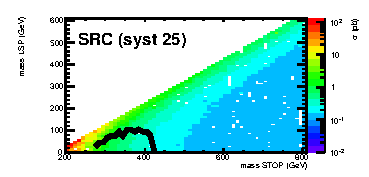
\includegraphics[width=0.5\linewidth]{plots/stopPlot/masses_SRC_xsecP.pdf}%
%        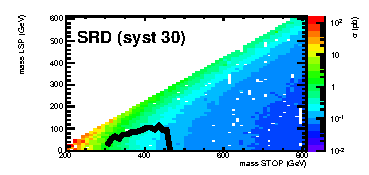
\includegraphics[width=0.5\linewidth]{plots/stopPlot/masses_SRD_xsecP.pdf}
%        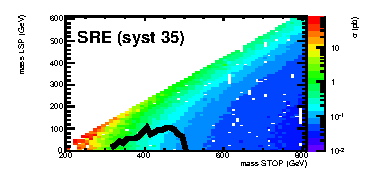
\includegraphics[width=0.5\linewidth]{plots/stopPlot/masses_SRE_xsecP.pdf}%
%        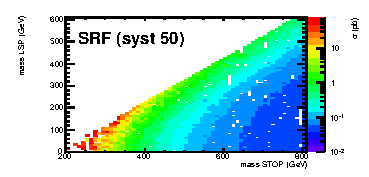
\includegraphics[width=0.5\linewidth]{plots/stopPlot/masses_SRF_xsecP.pdf}
%        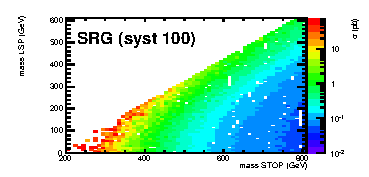
\includegraphics[width=0.5\linewidth]{plots/stopPlot/masses_SRG_xsecP.pdf}%
%    \caption{Expected upper limit on the cross section for the
%      T2tt. A less optimistic scenario is considered as systematics on the
%      background. (compared to Fig~\ref{fig:limO}).
%The assumed uncertainties on the background (in percent) is indicated on the plots.}
%\label{fig:limP}
%      \end{center}
%\end{figure}

\clearpage
